% Options for packages loaded elsewhere
\PassOptionsToPackage{unicode}{hyperref}
\PassOptionsToPackage{hyphens}{url}
%
\documentclass[
]{book}
\usepackage{lmodern}
\usepackage{amsmath}
\usepackage{ifxetex,ifluatex}
\ifnum 0\ifxetex 1\fi\ifluatex 1\fi=0 % if pdftex
  \usepackage[T1]{fontenc}
  \usepackage[utf8]{inputenc}
  \usepackage{textcomp} % provide euro and other symbols
  \usepackage{amssymb}
\else % if luatex or xetex
  \usepackage{unicode-math}
  \defaultfontfeatures{Scale=MatchLowercase}
  \defaultfontfeatures[\rmfamily]{Ligatures=TeX,Scale=1}
\fi
% Use upquote if available, for straight quotes in verbatim environments
\IfFileExists{upquote.sty}{\usepackage{upquote}}{}
\IfFileExists{microtype.sty}{% use microtype if available
  \usepackage[]{microtype}
  \UseMicrotypeSet[protrusion]{basicmath} % disable protrusion for tt fonts
}{}
\makeatletter
\@ifundefined{KOMAClassName}{% if non-KOMA class
  \IfFileExists{parskip.sty}{%
    \usepackage{parskip}
  }{% else
    \setlength{\parindent}{0pt}
    \setlength{\parskip}{6pt plus 2pt minus 1pt}}
}{% if KOMA class
  \KOMAoptions{parskip=half}}
\makeatother
\usepackage{xcolor}
\IfFileExists{xurl.sty}{\usepackage{xurl}}{} % add URL line breaks if available
\IfFileExists{bookmark.sty}{\usepackage{bookmark}}{\usepackage{hyperref}}
\hypersetup{
  pdftitle={A supervision guide for AAU Economics students},
  pdfauthor={Robert Smith},
  hidelinks,
  pdfcreator={LaTeX via pandoc}}
\urlstyle{same} % disable monospaced font for URLs
\usepackage{longtable,booktabs}
\usepackage{calc} % for calculating minipage widths
% Correct order of tables after \paragraph or \subparagraph
\usepackage{etoolbox}
\makeatletter
\patchcmd\longtable{\par}{\if@noskipsec\mbox{}\fi\par}{}{}
\makeatother
% Allow footnotes in longtable head/foot
\IfFileExists{footnotehyper.sty}{\usepackage{footnotehyper}}{\usepackage{footnote}}
\makesavenoteenv{longtable}
\usepackage{graphicx}
\makeatletter
\def\maxwidth{\ifdim\Gin@nat@width>\linewidth\linewidth\else\Gin@nat@width\fi}
\def\maxheight{\ifdim\Gin@nat@height>\textheight\textheight\else\Gin@nat@height\fi}
\makeatother
% Scale images if necessary, so that they will not overflow the page
% margins by default, and it is still possible to overwrite the defaults
% using explicit options in \includegraphics[width, height, ...]{}
\setkeys{Gin}{width=\maxwidth,height=\maxheight,keepaspectratio}
% Set default figure placement to htbp
\makeatletter
\def\fps@figure{htbp}
\makeatother
\setlength{\emergencystretch}{3em} % prevent overfull lines
\providecommand{\tightlist}{%
  \setlength{\itemsep}{0pt}\setlength{\parskip}{0pt}}
\setcounter{secnumdepth}{5}
\usepackage{booktabs}
\usepackage{amsthm}
\makeatletter
\def\thm@space@setup{%
  \thm@preskip=8pt plus 2pt minus 4pt
  \thm@postskip=\thm@preskip
}
\makeatother
\ifluatex
  \usepackage{selnolig}  % disable illegal ligatures
\fi
\usepackage[]{natbib}
\bibliographystyle{apalike}

\title{A supervision guide for AAU Economics students}
\author{Robert Smith}
\date{2021-05-10}

\begin{document}
\maketitle

{
\setcounter{tocdepth}{1}
\tableofcontents
}
\hypertarget{book-description}{%
\chapter{Book description}\label{book-description}}

This is a simple GitBook to assist students to write projects in partial fulfilment of the requirements of a degree in economics at Aalborg University.

\hypertarget{introduction-to-supervision}{%
\chapter{Introduction to supervision}\label{introduction-to-supervision}}

This is an introduction text that explains that I will be your
supervisor for your project and outlines some guidelines for our
collaboration.

As you can see from this text, my first language is English. So anyone
that wants to work on their English writing, or just get more exposure
to economics in English it might be a good opportunity for you -- If you
want to work outside of the country or in most multinationals here in DK
it is typically a requirement (Danmarks Nationalbank included). You will
not be assessed on your grammar, but you will need to make sense and
write in a professional manner.

If you would prefer to work in Danish, you are of course welcome to.

To get the most out of the supervision I recommend that in addition to
the introductory meeting, 3 group meetings should be sufficient.

0. \textbf{Introductory meeting:} We will go through literature search and a
few useful tools for writing in a collaborative project. (I will try to
do a digital/video guide so that you can watch / view / pause rewind the
info as much as you please.)

Here I will also try to get to understand where you are as a group in
terms of 5 main areas:

\begin{enumerate}
\def\labelenumi{\arabic{enumi}.}
\item
  Your subject specific knowledge (this till be in terms of the
  specific topic that you have chosen to work on).
\item
  Your experience and knowledge of group project work.
\item
  Your skills in project and process management for getting the job
  done.
\item
  Your technical academic skills -- Theory of science, methodology,
  methods and theory.
\item
  Your project writing skills -- The practical writing tools,
  reference mangers, programming skills, collaboration tools etc.
\end{enumerate}

1. \textbf{Meeting 1:} You need to have worked on and bring a complete
problem statement (see the guide and tips below), we will discuss it in
the first meeting.

2. \textbf{Meeting 2:} The literature review, and expected method should be
done, and any data or materials you plan to use should be collected. We
will go through your planned method and argumentation in the meeting.

3. \textbf{Meeting 3:} The analysis should be complete, and you should have
some working points for your discussion / conclusions. We will go
through your arguments verbally, and I will probe any major gaps I see
in your thinking.

\hypertarget{guidelines-for-supervision}{%
\chapter{Guidelines for supervision}\label{guidelines-for-supervision}}

\begin{enumerate}
\def\labelenumi{\arabic{enumi}.}
\item
  Any team member can communicate with me via Teams on behalf of your
  group. I expect that all communication has been discussed an
  agreed upon.
\item
  Just as you can expect me to read and provide comments on the days
  of meetings, I expect you to respect the deadlines you choose.

  \begin{enumerate}
  \def\labelenumii{\alph{enumii}.}
  \tightlist
  \item
    If you want something read before the meeting, it must be sent
    to me \textbf{at least 2 working days before the meeting}, \textbf{I.e.
    Midnight Thursday for a Monday meeting}. (Max 10 pages per
    meeting)
  \end{enumerate}
\item
  I will read and comment generally on the work but \textbf{will not make
  decisions for you}. Your ability to choose and apply the correct
  methods is part of what you will be assessed on.
\item
  Each meeting is planned for one hour.
\item
  \textbf{\underline{For every meeting you should bring with:}}

  \begin{enumerate}
  \def\labelenumii{\alph{enumii}.}
  \item
    Your problem statement (as it evolves with your work).
  \item
    A list of literature that you have covered up to that point
    (only the literature you have already read).
  \item
    Any additional formalities (this will depend on how big your
    group is).
  \end{enumerate}
\item
  The date by which you will be ready for the next meeting.
\end{enumerate}

\hypertarget{examinations}{%
\section{Examinations}\label{examinations}}

You can write and be examined in Danish or English. If you choose
Danish, it might be the case that one of our Danish speaking staff will
join in the examination, 1x external examiner + me + possibly 1x Danish
AAU examiner. This will depend on departmental resources, but you will
not be disadvantaged in any way because of any limitations that I might
have with the Danish language.

\hypertarget{leave-periods-absenteeism}{%
\section{Leave periods (absenteeism)}\label{leave-periods-absenteeism}}

I will be away from Aalborg for the following periods:

\begin{enumerate}
\def\labelenumi{\arabic{enumi}.}
\tightlist
\item
  Weeks 13 and 14. Thursday 2021/03/25 to Monday 2021/04/12.
\end{enumerate}

\hypertarget{teaching-and-time-pressures}{%
\section{Teaching and time pressures}\label{teaching-and-time-pressures}}

I will be teaching Mathematics 2 on each Wednesday of weeks 17, 18, and
19 -- for these weeks the best days to meet will be Thursday or Friday.

\hypertarget{rough-guide-to-project-structures}{%
\section{Rough guide to project structures}\label{rough-guide-to-project-structures}}

This is a \textbf{very rough} guide to writing a project. It is intended to
give you a very basic idea of what to include in a good project.

In terms of pages, each group will know how many people they have, the
official \textbf{maximum number of pages} (by character count, 2400
key-strokes including spaces) are:

1 Person: 15 pages

2 People: 25 pages

3 People: 35 pages

4 People: 40 pages

\textbf{Filling the pages is not the goal}, and you will not be given a
higher grade for filling all of your allocated pages with pointless
text. You will also not be penalised if you can get your message across
clearly in fewer pages. Keep in mind, that the average journal article
is roughly 15 -- 25 double spaced pages (around 8000 words).

You only need to address \textbf{one} problem, and to do it as well as
possible.

The written project is intended \textbf{to communicate} that you have done
your homework on your subject. This means that as a student \textbf{you should
be able to demonstrate that you}:

\begin{enumerate}
\def\labelenumi{\arabic{enumi}.}
\item
  Can identify an economic problem (or gap in the literature) that you
  think needs to be addressed (and why?!).
\item
  Can find, read and understand literature about the problem, and how
  others have dealt with it (reading and organising literature).
\item
  Can find the relevant information or data that you need to assess
  the problem, and that you know what to do with it when you do find
  it (number 2 helps with this) (data and methods).
\item
  Can present your findings in a well written document, where you give
  credit to all the authors that helped you to understand the
  problem (references).
\item
  If you make a statement, you either need to back it up with your own
  evidence, or someone else's.
\end{enumerate}

Compressing all of that into 8000 words is much more challenging than
filling 40 pages with unnecessary text and graphics. It also requires
much more cooperation on and discussion of what needs to go into those
pages to make them as effective as possible.

A good group member is one that can read a piece of writing critically
and give constructive feedback -- to do this effectively is necessary
for all group members to be clear about the ``red thread'' in the project
(the ``why'').

\textbf{I would personally prefer that you write about 15 pages of really good
work than 40 pages of low-quality work.}

\hypertarget{for-a-journal-article-size-paper-these-are-some-rough-guidelines}{%
\section{For a journal article size paper these are some rough guidelines:}\label{for-a-journal-article-size-paper-these-are-some-rough-guidelines}}

The share of pages between the sections depends on how much space you
\emph{need}. I say \emph{need}, because people reading your work want to get the
clearest message, in as few words as possible. A (very) rough guide as
to how many (academic) references each section could have is included in
red text.

\begin{enumerate}
\def\labelenumi{\arabic{enumi}.}
\item
  Abstract (+-150 words)
\item
  Introduction (0.75 -- 1.25 pages) (Motivation, justification,
  explanation of why? (4 -- 5 references))
\item
  Literature / theory (1.5 -- 3 pages, depending on how theoretical
  your paper is) (Demonstrate reading (6 -- 12 references))
\item
  Method (0.75 -- 3 pages, depending on how complex the explanation
  needs to be) (Justify choice, explain details (4 -- 5 references))
\item
  Results (1 -- 3 pages) (Presentation of results (2 -- 5 references))
\item
  Discussion (2 -- 5 pages) (Interpretations, comparisons,
  perspectives (4 -- 5 references))
\item
  Conclusion (1 page) (Link discussion to introduction (No new
  references))
\end{enumerate}

(The max pages in this example is 16.5 pages -- it is just an example,
and the split between the sections will change depending on the type of
research.)

(Min references in this example is 20, but this is on the high side. You
won't have time to read as much as that. 8 -- 15 references in total
should be enough if you find some really good ones.)

Keep it simple! That is the best advice I ever got. . . and the hardest
to follow, because you really need to be sure of what you're talking
about to write clearly and simply.

\hypertarget{time-planning-and-limitations}{%
\chapter{Time planning and limitations}\label{time-planning-and-limitations}}

Be aware of the time you have left to do the research. Data /
information collection and organisation takes time, and you need to get
started on it early if you want to be able to say anything useful by the
time you finish writing your project up. If you are efficient in how you
work this guide might help:

\textbf{A brief guide:}

\begin{enumerate}
\def\labelenumi{\arabic{enumi}.}
\item
  Problem identification and reading: 1 week
\item
  Write literature review: 1 week
\item
  Write first draft of introduction: 2 days
\item
  Data collection: 1 week
\item
  Write method and methodology section: 3 days
\item
  Data cleaning and analysis: 2 weeks
\item
  Write results: 1 week
\item
  Write conclusion: 2 days
\item
  Re-write introduction: 2 days
\item
  Check document for references and errors: 1 day
\end{enumerate}

Total: 8 weeks. From mid-March this would get you to mid-May, or from
mid-September it would take you to mid-November.

The later you start, the later you finish, or\ldots{} if you have a
deadline\ldots{} the more you have to sacrifice in terms of quality.

Remember to add time for:

\begin{itemize}
\tightlist
\item
  Reading and feedback
\end{itemize}

\hypertarget{reverse-time-planning}{%
\section{Reverse time-planning}\label{reverse-time-planning}}

A very powerful way to plan your project is to take the delivery date
and work backwards.

Pick your delivery date, and then work out how much time you need for
each of the jobs you need to do -- but starting from the last job first.

I will also share a project planner with you all when we have shared
supervision space established.

\hypertarget{data-sources-for-project-inspiration}{%
\chapter{Data sources for project inspiration}\label{data-sources-for-project-inspiration}}

\hypertarget{diverse-datasets}{%
\section{Diverse datasets}\label{diverse-datasets}}

\begin{enumerate}
\def\labelenumi{\arabic{enumi}.}
\tightlist
\item
  The Harvard Dataverse

  \begin{itemize}
  \tightlist
  \item
    \url{https://dataverse.harvard.edu/dataverse/harvard}
  \end{itemize}
\item
  Kaggle - datasets used for machine learning and AI applications

  \begin{itemize}
  \tightlist
  \item
    \url{https://www.kaggle.com/datasets}
  \end{itemize}
\item
  The New York Times Github repository

  \begin{itemize}
  \tightlist
  \item
    \url{https://github.com/nytimes}
  \end{itemize}
\item
  FiveThirtyWight Github page

  \begin{itemize}
  \tightlist
  \item
    \url{https://github.com/fivethirtyeight}
  \end{itemize}
\item
  The MIT Observatory of Economic Complexity - Economic trade data

  \begin{itemize}
  \tightlist
  \item
    \url{https://oec.world}
  \end{itemize}
\item
  The Google public data explorer (run in Chrome)

  \begin{itemize}
  \tightlist
  \item
    \url{https://www.google.com/publicdata/directory}
  \end{itemize}
\item
  European Union Open Data portal

  \begin{itemize}
  \tightlist
  \item
    \url{https://data.europa.eu/euodp/en/data/}
  \end{itemize}
\item
  Luxumborg income database

  \begin{itemize}
  \tightlist
  \item
    \url{https://www.lisdatacenter.org/our-data/}
  \end{itemize}
\end{enumerate}

\hypertarget{economic-time-series-databases}{%
\section{Economic time-series databases}\label{economic-time-series-databases}}

\begin{enumerate}
\def\labelenumi{\arabic{enumi}.}
\tightlist
\item
  The Bank for International Settlements

  \begin{itemize}
  \tightlist
  \item
    \url{https://www.bis.org/statistics/index.htm}
  \end{itemize}
\item
  OECD - stat-bank

  \begin{itemize}
  \tightlist
  \item
    \url{https://stats.oecd.org}
  \end{itemize}
\item
  AMECO - Annual macroeconomic of the European Commission's Directorate General for Economic and Financial Affairs

  \begin{itemize}
  \tightlist
  \item
    \url{https://ec.europa.eu/info/business-economy-euro/indicators-statistics/economic-databases/macro-economic-database-ameco_en}
  \end{itemize}
\item
  The World Bank open data source

  \begin{itemize}
  \tightlist
  \item
    \url{https://data.worldbank.org}
  \item
    Sub-components for microdata, DataBank and a data catalogue
  \end{itemize}
\item
  Eurostat Database

  \begin{itemize}
  \tightlist
  \item
    \url{https://ec.europa.eu/eurostat/data/database}
  \end{itemize}
\item
  Danish Data - Kim Abildgren's historical database

  \begin{itemize}
  \tightlist
  \item
    \url{https://sites.google.com/view/kim-abildgren/historical-statistics}
  \end{itemize}
\item
  Jorda-Schularick-Taylor Macrohistory Database

  \begin{itemize}
  \tightlist
  \item
    \url{http://www.macrohistory.net/data/}
  \end{itemize}
\end{enumerate}

\hypertarget{rough-guide-to-writing-a-problem-statement}{%
\chapter{Rough guide to writing a problem statement}\label{rough-guide-to-writing-a-problem-statement}}

Coming up with a good question does not mean coming up with a question
that will change the world. It means coming up with a question that you
can answer \textbf{in the time you are allowed}, and \textbf{with the tools you
have (or have time to learn)}.

A note on how to get started with your problem selection -- try to be
curious. It is going to take some active effort.

\textbf{Most of you have identified an area of interest, rather than any
specific question.} These are just a few pointers to help you to
identify a good problem.

\begin{itemize}
\tightlist
\item
  If you want to read a pretty good ``how-to'' guide, try this one:
  \url{https://www.wikihow.com/Write-a-Problem-Statement}
\end{itemize}

You need to actively apply yourselves to \emph{finding} a question:

\hypertarget{step-1-brainstorm-ideation}{%
\section{Step 1: Brainstorm / ideation}\label{step-1-brainstorm-ideation}}

\begin{itemize}
\item
  Find a meeting room and mind-map an area of economics that you are
  interested in.
\item
  A very high-level overview of the courses (like the table of
  contents in your textbooks) you have done so far should help you to
  understand the tools that you have, which you can use to answer
  whatever question you end up asking.

  \begin{itemize}
  \tightlist
  \item
    Some of these tools will be theories, models, data types and
    sources. The learning outcomes of your courses are also a good
    guide (check Moodle).
  \end{itemize}
\item
  If you really want to be active in your search for problems, and
  deal with real life issues -- pick up a phone and make some calls to
  people in the area or industry you want to look at. These kinds of
  discussion can be really motivating and insightful.
\item
  As a group you can really benefit by getting ideas and input from
  each other. This does not need to take a long time but does require
  effort.
\item
  Don't get caught up by not deciding what to do -- get into a room,
  set a time frame and get finished with the choice early.
\end{itemize}

Some interesting possible approaches can be seen here -- many of these
are related to innovation to products, but the general ideas can be used
to create research ideas too:

\begin{itemize}
\item
  ``The 7 All-time Greatest Ideation Techniques''

  \begin{itemize}
  \tightlist
  \item
    \url{https://innovationmanagement.se/2013/05/30/the-7-all-time-greatest-ideation-techniques/}
  \end{itemize}
\item
  ``The master ideation toolbox - 10 tools to unleash creativity from
  anyone.''

  \begin{itemize}
  \tightlist
  \item
    \url{https://uxdesign.cc/the-master-online-ideation-toolbox-part-1-2-47401c3ad861}
  \end{itemize}
\item
  ``Our favorite ideation tools''

  \begin{itemize}
  \tightlist
  \item
    \url{https://www.boardofinnovation.com/staff_picks/our-favorite-ideation-tools/}
  \end{itemize}
\item
  ``Ideation in Design Thinking: Tools and Methods'' - 05/02/2017 - by
  Rafiq Elmansy

  \begin{itemize}
  \tightlist
  \item
    \url{https://www.designorate.com/ideation-design-thinking-tools/}
  \end{itemize}
\end{itemize}

\hypertarget{digital-tools-for-getting-your-project-started}{%
\subsection{Digital tools for getting your project started}\label{digital-tools-for-getting-your-project-started}}

There are a heap of tools available:

\hypertarget{tools-that-can-help-with-brainstorming-and-project-management}{%
\subsubsection{Tools that can help with brainstorming and project management}\label{tools-that-can-help-with-brainstorming-and-project-management}}

\begin{enumerate}
\def\labelenumi{\arabic{enumi}.}
\tightlist
\item
  Trello board
\item
  Padlet
\item
  Notion
\item
  Prezi
\item
  Wonder
\item
  Mural
\end{enumerate}

\hypertarget{tools-that-can-help-with-content-creation-for-questionnaires-interactive-quizzes}{%
\subsubsection{Tools that can help with content creation for questionnaires / interactive quizzes}\label{tools-that-can-help-with-content-creation-for-questionnaires-interactive-quizzes}}

\begin{enumerate}
\def\labelenumi{\arabic{enumi}.}
\tightlist
\item
  \href{https://www.mentimeter.com}{Mentimeter}
\item
  \url{Peergrade}
\item
  MS Forms (\href{https://www.loom.com/share/ed2fd65abfd64189b2c81f8daff7ec79}{Integration of Forms with Teams and OneDrive})
\item
  \href{https://www.fyrebox.com}{Fyrebox}
\item
  \href{https://coggle.it}{Coogle}
\item
  \url{Kahoot}
\end{enumerate}

\hypertarget{communication-tools-for-collaboration}{%
\subsubsection{Communication tools for collaboration}\label{communication-tools-for-collaboration}}

\begin{enumerate}
\def\labelenumi{\arabic{enumi}.}
\tightlist
\item
  OSX apple screen sharing (with control option)
\item
  OSX Facetime
\item
  MS Teams
\item
  Facebook messenger
\item
  Disqord
\item
  Skype / Skype for business
\item
  Whatsapp
\end{enumerate}

\hypertarget{additional-learning-tools-for-self-learning-or-training}{%
\subsubsection{Additional learning tools for self-learning or training}\label{additional-learning-tools-for-self-learning-or-training}}

\begin{enumerate}
\def\labelenumi{\arabic{enumi}.}
\tightlist
\item
  \href{https://www.datacamp.com}{DataCamp}
\item
  \href{https://www.khanacademy.org}{Khan Academy}
\item
  \href{https://www.udemy.com}{Udemy}
\item
  \href{https://www.coursera.org}{Coursera}
\item
  \href{https://www.edx.org}{Edx}
\item
  \href{https://analytics.google.com/analytics/academy/}{Google Analytics Academy}
\item
  \href{https://docs.microsoft.com/en-gb/learn/powerplatform/power-bi?WT.mc_id=sitertzn_learntab_guidedlearning-card-powerbi}{Microsoft Learn - For Power BI}
\end{enumerate}

\hypertarget{courses-in-econometrics-at-aau}{%
\subsection{Courses in Econometrics at AAU}\label{courses-in-econometrics-at-aau}}

The following main methods are covered in each of the semesters, and economic analyses should be conducted that reflect a knowledge up to at least the level of technical analysis of each semester.

\hypertarget{methods-notes---econometrics-4.-semester}{%
\subsubsection{Methods notes - Econometrics 4. semester}\label{methods-notes---econometrics-4.-semester}}

\begin{enumerate}
\def\labelenumi{\arabic{enumi}.}
\tightlist
\item
  OLS - simple linear regression
\item
  OLS - multiple linear regression
\item
  Linear regressions in matrices
\item
  Inference and hypothesis testing
\item
  And 6. OLS - Assymptotics, functional form and prediction

  \begin{enumerate}
  \def\labelenumii{\arabic{enumii}.}
  \tightlist
  \item
    Goodness of fit
  \end{enumerate}
\item
  Multiple regression analysis with qualitative data

  \begin{enumerate}
  \def\labelenumii{\arabic{enumii}.}
  \tightlist
  \item
    Using dummy variables
  \end{enumerate}
\item
  Heteroskedasticity.
\item
  Normal distribution model specification.

  \begin{enumerate}
  \def\labelenumii{\arabic{enumii}.}
  \tightlist
  \item
    Proxy variables measure error.
  \end{enumerate}
\item
  Non-nested models, missing data, outliers, least absolute deviations, estimations and multicollinearity.
\item
  Instrumental variables - 2 stage least squares.
\item
  Instrumental variables continued - 2 stage least squares with heteroskedasticity.
\item
  PROBIT and LOGIT
\end{enumerate}

\hypertarget{methods-notes---econometrics-5.-semester}{%
\subsubsection{Methods notes - Econometrics 5. semester}\label{methods-notes---econometrics-5.-semester}}

\begin{enumerate}
\def\labelenumi{\arabic{enumi}.}
\tightlist
\item
  Time series and seasonality trends
\item
  Cyclical correlation in univariate time-series
\item
  AR and MA processes

  \begin{enumerate}
  \def\labelenumii{\arabic{enumii}.}
  \tightlist
  \item
    ACF and PACF
  \end{enumerate}
\item
  Stationarity
\item
  ARIMA - Autoregressive Integrated Moving Average Model
\item
  Mandatory exercise in forecasting

  \begin{enumerate}
  \def\labelenumii{\arabic{enumii}.}
  \tightlist
  \item
    Properties and evaluation
  \end{enumerate}
\item
  Multivariate time series analysis

  \begin{enumerate}
  \def\labelenumii{\arabic{enumii}.}
  \tightlist
  \item
    Engel-Granger
  \item
    ARDL - Auto-regressive distributed lag models
  \end{enumerate}
\item
  Dynamic models with non stationary variables

  \begin{enumerate}
  \def\labelenumii{\arabic{enumii}.}
  \tightlist
  \item
    Cointegration and error correction models
  \item
    Spurious regression
  \end{enumerate}
\item
  Further extension

  \begin{enumerate}
  \def\labelenumii{\arabic{enumii}.}
  \tightlist
  \item
    Cointegration and bounce test
  \end{enumerate}
\item
  VAR

  \begin{enumerate}
  \def\labelenumii{\arabic{enumii}.}
  \tightlist
  \item
    Vector
  \end{enumerate}
\end{enumerate}

\hypertarget{step-2-getting-that-problem-statement-clear}{%
\section{Step 2: Getting that problem statement clear}\label{step-2-getting-that-problem-statement-clear}}

\textbf{Where to start?}

Read. This starts with a good literature search.

Some reflective questions that I recommend you consider before the meeting:

\begin{enumerate}
\def\labelenumi{\arabic{enumi}.}
\item
  \textbf{What are you investigating (you have a problem statement for this already - but it still lacks some clarity)?}\\
  i.e.
  What do you mean by: ``årsagen''?
  What do you mean by: ``handel med omverden''?
  How do you define globalisation?
  When you say ``påvirke'', what do you mean?\\
  ~\\
  Is it all people in the USA? All industries? Aggregate economic measures?\\
  When you talk about effects, it usually implies that there is some kind of causal relationship\ldots{} When looking at national economic aggregates - there are many possible ``causes'' for changes. Political, social, economic, technological, etc.
\item
  \textbf{Why is it important to investigate this?}
\item
  Who would care about this result? i.e.~why are you doing this research? what is the motivation behind finding an answer to this question?
\item
  What is the problem that you are actually trying to throw some light on?
\item
  \textbf{How have others explored this?}

  \begin{enumerate}
  \def\labelenumii{\arabic{enumii}.}
  \item
    What did they find?
  \item
    What are some of the conclusions that have been drawn?
  \item
    Are there some concerns/issues with how other people have investigated it?
  \end{enumerate}
\item
  \textbf{How could you possibly explore this question?}

  \begin{enumerate}
  \def\labelenumii{\arabic{enumii}.}
  \item
    Are there some alternative explanations that have not been considered?
  \item
    Are there some other perspectives that have been ignored? For example\ldots{} if the USA is able to strengthen it's trade position, what are the consequences for smaller countries that compete in the same markets?
  \item
    Is there some new data available that illuminates a new part of the problem?
  \item
    Are there better measures available for inequality / trade performance / competitiveness / etc. ?
  \end{enumerate}
\item
  \textbf{How are you going to make the choice about what road to take?}

  \begin{enumerate}
  \def\labelenumii{\arabic{enumii}.}
  \item
    If you had all the money and time in the world, how would you investigate this problem?
  \item
    What are the first steps / minimum requirements needed to be able to answer the question?
  \item
    What options are real possibilities in the time that is left?
  \item
    Who is going to do what?
  \end{enumerate}
\end{enumerate}

\hypertarget{using-the-introduction-as-the-route-to-the-problem-statement}{%
\section{Using the introduction as the route to the problem statement}\label{using-the-introduction-as-the-route-to-the-problem-statement}}

A good introduction leads to a good problem statement, but this is only
possible if you have some good material to work with.

\hypertarget{example-flow-of-a-good-introduction}{%
\subsection{Example flow of a good introduction}\label{example-flow-of-a-good-introduction}}

\begin{enumerate}
\def\labelenumi{\arabic{enumi}.}
\item
  You could list some shocking figures or numbers that highlight that
  there is some area / issue that we should be concerned about. It
  could also be some clear contradiction or controversy in the
  literature that needs clarification - but this requires some careful
  reading. (This defines the problem area that you want to address -
  normally these are the effects of some other problem that can be
  identified.)
\item
  You could then explain that some people see (explain) these
  facts/figures from the perspective of A / B / C . . . and conclude
  that X / Y / Z. Another group of researchers suggest that there may
  be another way to interpret these figures.. they say. . . etc. (This
  highlights existing theories in the literature - these could be
  conflicting explanations for the effects that are observed by
  different researchers. Always remember that research can have a
  particular agenda, i.e.~to promote efficiency of markets, or to
  critique main-stream literature - so be a little critical when
  reading. Every researcher is trying to sell their ideas.)
\item
  Next, you could explain that `these' different approaches suggest
  that this problem could be investigated by doing E/F/G.
  (Identification of possible ways of addressing the issue - There are
  a variety of quantitative and qualitative methods, and some people
  rely more on some than on others. This section should still be able
  to refer to how other people have addressed the issue. Here is where
  you narrow down what might be a good way to look at the problem.)
\item
  More specifically, therefore, we want to investigate how / if / what
  the effects of / etc. (By this stage you should be able to be
  specific about the exact part of the problem that you are interested
  in addressing, and all of the arguments for why it is interesting
  should already have been made.)
\end{enumerate}

\hypertarget{some-general-notes-about-writing-a-problem-statement}{%
\section{Some general notes about writing a problem statement}\label{some-general-notes-about-writing-a-problem-statement}}

The general structure of questions in most economic analyses is: What
is, has been, or will be the impact of \textbf{A} on \textbf{B}?

\hypertarget{where-do-you-find-a-problem-in-macroeconomics}{%
\subsection{Where do you find a problem in macroeconomics?}\label{where-do-you-find-a-problem-in-macroeconomics}}

Many economic queries attempt to measure social consequences, and most
often try to assign a financial value to those consequences. Sometimes
this is phrased as a ``comparative outcome'' or ``alternative scenario''.
Normally this means that one option is \emph{better} than another. This is
not surprising, since pretty much all macroeconomic variables are
aggregated financial values or derivatives thereof.

Other ways to frame a question could be:

\begin{enumerate}
\def\labelenumi{\arabic{enumi}.}
\item
  Why is one option better than the other? How can you tell?
\item
  How does a change in X affect income for the economy / households /
  teachers?
\item
  How many people are employed?
\item
  Labour productivity?
\item
  How is the standard of living affected?
\end{enumerate}

These are justification options (evidence) to motivate \emph{why} an
investigation is a good idea. Just remember that you need to be able to
find the evidence to back up your arguments. As noted in the example of
an introduction flow above, your selection of a method should be the
logical conclusion of your reading.

\hypertarget{answering-the-why}{%
\subsection{Answering the Why?}\label{answering-the-why}}

Why is it that investigating this problem will be beneficial? To answer
the question generally requires awareness of:

\begin{enumerate}
\def\labelenumi{\arabic{enumi}.}
\item
  What?
\item
  When?
\item
  Where?
\item
  Who?
\item
  In what way?
\item
  How?
\end{enumerate}

These things are the specifics of the problem statement, but they will
not provide you with the answer to why it is important.

The best place to find an answer to \emph{why?} is to read some of the most
recent work on the topic you have found. Anything that has been
published has been read and edited by at least 5 people by the time it
goes to a journal. The arguments in those articles should therefore be
pretty reasonable.

Once you understand your \emph{why?} you can start with the specifics

\hypertarget{what}{%
\subsection{What?}\label{what}}

For example: If you chose to research currency markets, some of the
sub-categories could be (What?):

\begin{itemize}
\item
  Trading platforms
\item
  Exchange rate policies
\item
  Regulations
\item
  Common currency areas
\item
  Clearing and settlement systems
\item
  Speculation
\item
  Risk-mitigation / hedging
\end{itemize}

This delimitation is often determined by the problem area that you
identify. Normally illustrated by something interesting or concerning,
which leads you to think that investigating the area might be
interesting.

You can go the other way around, and check what has been written about recently or is
currently being funded at the EU or national levels. Read some of the
latest literature relating to it and then identify if there is a similar
problem in an area that has not yet been investigated.

A third possibility is to open up some of the really amazing data
repositories of major institutions and see if some of those can inspire
you.

\hypertarget{when}{%
\subsection{When?}\label{when}}

You need to be carefully aware of what time period you choose to
investigate, as it has direct consequences for the types of conclusions
you can make from your analysis. If you look at 1950 -1970 consumption
data, you can't really say anything intelligent about the use of
disposable income in 2020.

Historical analysis is crucial in economics, but you should always be
aware of how the structure of the economies of the world have shifted
over time.

Education rates, the type of institutions that exist, levels of
unemployment, the size of government, etc.

A trendy catch phrase for this kind of context is PESTLE, an anagram for
how the context of countries change:

\begin{enumerate}
\def\labelenumi{\arabic{enumi}.}
\item
  Political
\item
  Economic
\item
  Social
\item
  Technological
\item
  Legal
\item
  Environmental
\end{enumerate}

Please \textbf{don't write this list out and do a PESTLE analysis} in your
projects, it is just to tell you that there are many changes that take
place over time. And that you need to think specifically about time in
your problem statement.

\hypertarget{where}{%
\subsection{Where?}\label{where}}

This is quite obvious but is not only related to geographical borders.
For example, a study could be:

\begin{itemize}
\item
  National
\item
  Municipal
\item
  Regional
\item
  Global
\item
  Local (or micro)
\end{itemize}

\hypertarget{who}{%
\subsection{Who?}\label{who}}

Which groups are involved in your project, and who is it that will be
interested in reading the results of your research? Who will the
research / problem investigation be useful or interesting for.

\begin{itemize}
\item
  Demographic specific (Ex., students, low-income families, employees
  at public institutions)
\item
  Institution specific (Ex. Banks, the national bank, the stock
  exchange, or one specific institution)
\item
  Industry specific (Ex. Mining, agriculture, home owners
  associations, mortgage institutes, or alternatively at a ``sector''
  level, such as households, firms, government etc.)
\item
  Country specific
\item
  Etc.
\end{itemize}

\hypertarget{in-what-way}{%
\subsection{In what way?}\label{in-what-way}}

You also need to know what kind of impact or relationship you are
looking for. Is it,

\begin{itemize}
\item
  \emph{How much of the behaviour of A can be explained by B}?
\item
  Is it a \emph{theoretical or empirical issue} or are you interested in?
\item
  Or \emph{how much influence will A have on B? Or vice versa, or both}?
\item
  Is it causal? Are you arguing that one thing is \emph{causing} another
  thing? -- you have to be quite careful trying to do these ones.
\end{itemize}

\hypertarget{how}{%
\subsection{How?}\label{how}}

Finally, you need to be able to explain how you are going to investigate
the problem. You should consider your tools and your course on
methodology (and philosophy of science) to be able to figure out how
will you answer the question.

You can boggle your brain a bit with the wiki-page on philosophy of
science here:

\url{https://en.wikipedia.org/wiki/Philosophy_of_science}

Recall that methodology is layered, a very simplistic way to think about it is
as a hierarchy:

\begin{quote}
\textgreater{} Philosophy of science

-\textgreater{} Methodology

-\/-\textgreater{} Theory

-\/-\/-\/-\textgreater{} Methods
\end{quote}

\textbf{You can watch a few videos about what this is:}

\begin{enumerate}
\def\labelenumi{\arabic{enumi}.}
\item
  This one is pretty good, but a little dry:
  \url{https://youtu.be/IvwkMxgahA4}
\item
  Daniel Hausman - This one has some interesting perspectives (but is
  much better in 2x speed): \url{https://youtu.be/EfF6WD8s_ps} (but he
  doesn't really list any specific philosophies)
\item
  Paul Hoyningen-Huene at Leibniz Universität Hannover has a whole
  course on it if you get really caught up in it -
  \url{https://www.youtube.com/watch?v=tP8teUgZcBY\&list=PLGV2ddg-PFGvWKDeTyrUji7TXY8y1SHjl}
  (He is pretty entertaining and you could learn a lot in his course
  -- and have a few laughs at dad jokes -- in 22 lectures)
\item
  Marc Lavoie -- This might help if you are interested in locating the theory you are using in either heterodox or orthodox categories of economic methodology. Disclaimer: I do not believe this is a constructive way to categorise methodology, but it is a common way.
  \url{https://youtu.be/DEROFQIao4o}
\end{enumerate}

The philosophy of science defines what kind of results will be
considered valid. For example, is it valid to make a conclusion about
the future based on the past (i.e.~to use data to make predictions)?

Some examples of this are:

\begin{itemize}
\item
  Cartesian / Euclidian philosophies of science
\item
  The Babylonian mode of thinking
\item
  Critical realism
\item
  Scepticism
\item
  Logical positivism
\end{itemize}

This colour coded conceptual map of philosophy might put some of the
terms you come across into perspective (with some spin on ``education''):

\url{https://cmapspublic3.ihmc.us/rid\%3D1196256709922_36526043_8120/1196256715039I908793757I8261Iimage}

Theories use methods, and methods are part of a particular methodology,
and the methodology is made valid by the theory of science inside which
it fits.

Methods are at the bottom of the pyramid, and can be quantitative or
qualitative, or a combination of both. It is important to be aware of
what you are doing and using. They are normally used to motivate one or
another theory.

This stuff can be extremely dry and boring, or it can also be super
interesting (if you are into it). It is how we know, that we know, that
what we know, is really something factual -- or what a fact is in the
first place. It is closely related to metaphysics, epistemology and
ontology. None of which will help you cook an egg in the morning, but
you might find the study as fascinating as I do (even if I will never
suck up the energy to finish reading Immanuel Kant's \emph{Critique of Pure
Reason}).

This Saunders et al.~research onion is a pretty useful way to think
about each of the decisions we make when constructing out research.
Starting from the outside moving inwards:

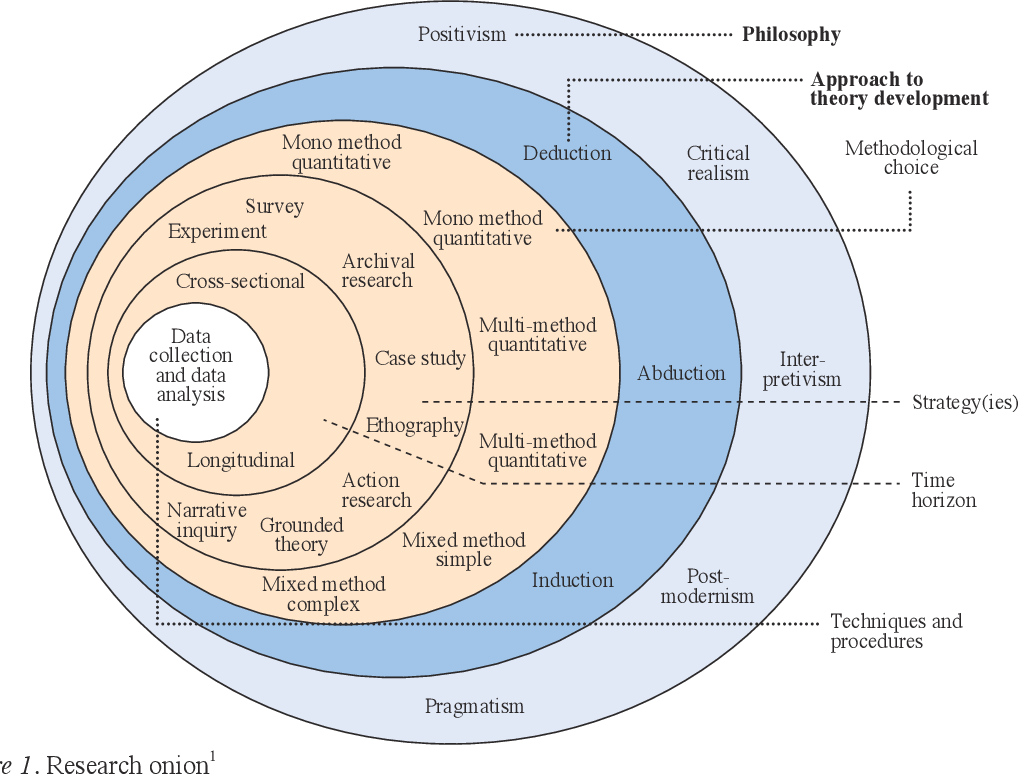
\includegraphics{images/onion.png}

Source: \href{https://www.researchgate.net/profile/Mark-Saunders-10/publication/330760964_Research_Methods_for_Business_Students_Chapter_4_Understanding_research_philosophy_and_approaches_to_theory_development/links/5c53056f299bf12be3f0e2cf/Research-Methods-for-Business-Students-Chapter-4-Understanding-research-philosophy-and-approaches-to-theory-development.pdf}{Saunders, Lewis and Thornhill (2019), Research methods for
business
students}

\hypertarget{alternative-platforms-for-writing-projects}{%
\chapter{Alternative platforms for writing projects}\label{alternative-platforms-for-writing-projects}}

This is a brief list of options when writing a project. Some options are best suited to complex data work, such as Rmarkdown, whereas others are better suited to collaborative writing, such as Overleaf, MS Word via MS Teams.

Each of these platforms are presented in short videos below. There are some clear advantages to using some rather than others. For each you will need to have some knowledge about how the program works in order to use it, and this might require a time investment.

My preference is to recommend open-source options that allow for efficient collaboration and / or reproducible research.

\textbf{Free / open source options}

\begin{enumerate}
\def\labelenumi{\arabic{enumi}.}
\item
  Overleaf / LaTeX
\item
  RMarkdown
\item
  Google Docs (but you pay in terms of data security)
\end{enumerate}

\textbf{Paid / Subscription options}

\begin{enumerate}
\def\labelenumi{\arabic{enumi}.}
\tightlist
\item
  MS Word
\end{enumerate}

\hypertarget{overleaf-latex}{%
\section{Overleaf (LaTeX)}\label{overleaf-latex}}

Overleaf offers a number of excellent guides for getting started, but for those that would like an explanation from me of some of the basics, please feel free to watch the following videos.

One of the most powerful features of Overleaf is the ability to who any change is attributed to, and to roll back changes incrementally. This is possible due to the built in version control features that the platform offers.

\begin{enumerate}
\def\labelenumi{\arabic{enumi}.}
\item
  \href{https://www.youtube.com/watch?v=g8Ejj0T0yG4}{Video: How open an account in Overleaf}
\item
  \href{https://github.com/robabsmith/Example-project}{GitHub: Template documents and resources}
\item
  \href{https://www.loom.com/share/6d0d4f7108f041d082253c636a52dee8}{Video: Integration of Mendely with Overleaf}
\item
  \href{https://youtu.be/BAt5xYP70u0}{Integration of Git with Overleaf (Quite a heavy Spanish accent, but a good guide)}
\end{enumerate}

\hypertarget{rmarkdown}{%
\section{RMarkdown}\label{rmarkdown}}

RMarkdown is a derivative of Markdown syntax, and is a very simple way to write. The video guide below covers a lot of ground, and uses the GitHub template that follows as an example.

\begin{enumerate}
\def\labelenumi{\arabic{enumi}.}
\item
  \href{https://www.loom.com/share/407ae8d0f00e4a05941a9a09e5e13f96}{Video: Getting started with Rmarkdown}
\item
  \href{https://github.com/robabsmith/Rmarkdown-project-template}{GitHub: Project template for single or multi-file projects}
\end{enumerate}

\hypertarget{ms-word-via-ms-teams}{%
\section{MS Word via MS Teams}\label{ms-word-via-ms-teams}}

MS Word files can be dropped into the ``General'' chat area of any Team created using the MS Teams app. These files can then be edited simultaneously by all team members.

\hypertarget{reference-and-bibliography-management}{%
\chapter{Reference and bibliography management}\label{reference-and-bibliography-management}}

With the aid of technology, it is not possible to very easily and efficiently manage and utilise the literature sources that you need when writing an academic project.

The first step is finding the appropriate literature, which is explained in more detail in the chapter below. This section is included in advance as it is useful to select the bibliography management software in advance of completing a literature search.

Each of the more popular reference management software tools have a variety of advantages and disadvantages, depending on what program you choose to work in.

My own preferences are shaped by my experience with each program - and a desire to make sure that the content I create will be accessible to me always, regardless of whether I am at the university or not. If better options exist I would be most interested in hearing about them.

The first two software options enable in-text referencing and automatic generation of reference lists in MS word. The last option, of manually collecting your reference data, is the most inefficient, but has some benefits. The videos below will link to the \href{https://www.loom.com}{Loom} hosting service, and provide a guide to Mendely. Refworks can do pretty much everything that Mendeley can, but it is expensive to use once you leave the university.

\textbf{\textbf{Order of preference}}

\begin{enumerate}
\def\labelenumi{\arabic{enumi}.}
\item
  \href{https://www.mendeley.com/download-desktop-new/}{Mendeley}
\item
  \href{https://www.aub.aau.dk/software-web/refworks/}{Refworks}
\item
  \href{https://youtu.be/JwXQb25cpqA}{Manual storage}
\end{enumerate}

\hypertarget{videos-of-reference-software}{%
\section{Videos of reference software}\label{videos-of-reference-software}}

\begin{enumerate}
\def\labelenumi{\arabic{enumi}.}
\item
  \href{https://youtu.be/MiKbS01Aulo}{Video: Mendeley in 5 minutes: Part 1}
  \href{https://youtu.be/kSu4tO8Dwak}{Video: Mendeley in 5 minutes: Part 2}
  \href{https://youtu.be/XU3cjfY4G5s}{Video: Mendeley in 5 minutes: Part 3}
\item
  \href{https://youtu.be/XTfVCiksapk}{Use of in-text referencing in Ms Word}
\item
  \href{https://youtu.be/zkrVbBSrK_w}{In-text referencing, and creating a reference list in Ms Word}
\item
  \href{https://www.loom.com/share/6d0d4f7108f041d082253c636a52dee8}{Integration of Mendely and Overleaf}
\item
  \href{https://github.com/robabsmith/Example-project}{GitHub Example: Citation options and text edit options in Overleaf}
\item
  \href{https://www.loom.com/share/407ae8d0f00e4a05941a9a09e5e13f96}{Video: Reference lists in RMarkdown}
\item
  \href{https://www.loom.com/share/407ae8d0f00e4a05941a9a09e5e13f96}{Video: Citation options in RMarkdown (Same video as in 6. above)}
\end{enumerate}

\hypertarget{literature-searching}{%
\chapter{Literature searching}\label{literature-searching}}

Literature searches can be completed in a number of ways. There are several very useful free literature search options, as well as more expensive options that you will have access to as a university student.

\hypertarget{free-search-options}{%
\section{Free search options}\label{free-search-options}}

\begin{enumerate}
\def\labelenumi{\arabic{enumi}.}
\tightlist
\item
  \href{https://scholar.google.com}{Google Scholar}
\item
  \href{https://www.semanticscholar.org}{Semantic Scholar}
\end{enumerate}

\hypertarget{paid-search-options}{%
\section{Paid search options}\label{paid-search-options}}

These options are very effectively combined and the University library website. Where the \emph{Primo} service can be used to search a wide variety of databases for a specific search string (or phrase).

\begin{enumerate}
\def\labelenumi{\arabic{enumi}.}
\tightlist
\item
  \href{https://www.en.aub.aau.dk}{Aalborg University Universitetsbiblioteket}
\end{enumerate}

The university site also allows students to access each of the available underlying databases individually and use the special search features that are available for each. Several of these databases allow for bulk exportation of bibliographic information, and can be easily synchronised with referencing software described in the section above.

\begin{enumerate}
\def\labelenumi{\arabic{enumi}.}
\setcounter{enumi}{1}
\tightlist
\item
  \href{https://www.en.aub.aau.dk/find-material/databases}{Databases and suppliers}
\end{enumerate}

A short video introdution to literature search is included as a video reference below. This link will take you to a video recorded and stored on the \textbf{Loom} hosting platform.

\hypertarget{literature-search-videos}{%
\section{Literature search videos}\label{literature-search-videos}}

\begin{enumerate}
\def\labelenumi{\arabic{enumi}.}
\item
  \href{}{How to conduct an efficient literature search}
\item
  \href{}{How to construct the key search criteria for your literature search}
\item
  \href{}{How to save and export search results}
\end{enumerate}

\hypertarget{appendix-literature-search-construction}{%
\chapter{Appendix: Literature search construction}\label{appendix-literature-search-construction}}

\hypertarget{project-title}{%
\section{Project title}\label{project-title}}

Stock-flow consistent models -- property and mortgage

\hypertarget{description-of-subject}{%
\section{Description of subject}\label{description-of-subject}}

Stock flow consistent model to cover mortgage debt of the household sector

\hypertarget{problem-statement-for-project}{%
\section{Problem statement for project}\label{problem-statement-for-project}}

Debt to disposable income levels in several Danish sectors have risen to the highest ever recorded levels, while the Danish central bank (Danmarks nationalbank), the IMF and Finanstilsynet all report that there are no serious threats to financial stability. Financial deregulation, relaxation of borrowing criteria and product innovation have been cited as the leading causes of this trend. This thesis aims to explore credit creation and macro-financial risks related to the expansion of household debt in Denmark by examining institutional sector and individual household balance sheets.

\hypertarget{search-criteria-development-summary}{%
\section{Search criteria development -- summary}\label{search-criteria-development-summary}}

\begin{enumerate}
\def\labelenumi{\arabic{enumi}.}
\tightlist
\item
  Step 01: List all concepts
\item
  Step 02: Group words into ``Blocks'' of concepts
\item
  Step 03: Check for any synonyms
\item
  Step 04: Add Boolean operators
\item
  Step 05: Prioritise blocks according to subject
\item
  Step 06: Selection of appropriate databases
\item
  Step 07: Perform search block by block
\item
  Step 08: Combine search blocks
\item
  Step 09: Refine search parameters based on results
\item
  Step 10: Document search results and search limiters
\item
  Step 11: Compare results and refine search parameters
\item
  Step 12: Export final list of documents
\item
  Step 13: Repeat steps 07 to 12 for each database
\item
  Step 14: Remove duplicates identified from different databases
\item
  Step 15: Remove non-relevant documents based on title and abstract
\item
  Step 16: Read core literature
\item
  Step 17: From core reading, find and read any key literature identified by other authors.
\end{enumerate}

\hypertarget{search-criteria-development}{%
\section{Search criteria development}\label{search-criteria-development}}

\hypertarget{step-01-list-all-concepts}{%
\subsection{Step 01: List all concepts}\label{step-01-list-all-concepts}}

\begin{enumerate}
\def\labelenumi{\arabic{enumi}.}
\tightlist
\item
  Stock Flow Consistent Models
\item
  Structural Econometric Models
\item
  Mortgage debt
\item
  Housing market
\item
  Macroeconomic models
\item
  Post Keynesian theory
\item
  Denmark
\item
  Households
\item
  Sector balance analysis
\item
  Household debt
\end{enumerate}

\hypertarget{step-02-group-words-into-blocks-of-concepts}{%
\subsection{Step 02: Group words into ``Blocks'' of concepts}\label{step-02-group-words-into-blocks-of-concepts}}

\begin{enumerate}
\def\labelenumi{\arabic{enumi}.}
\tightlist
\item
  ``Stock Flow Consistent Models'' OR ``Structural Econometric Models'' OR ``Sector balance analysis''
\item
  ``Macroeconomic''
\item
  ``Mortgage debt'' OR ``Housing market''
\item
  ``Post Keynesian theory''
\item
  ``Denmark''
\item
  ``Households''
\item
  ``debt'' OR Credit''
\end{enumerate}

\hypertarget{step-03-check-for-any-synonyms-and-use-ms-word-to-check-for-spelling-errors}{%
\subsection{Step 03: Check for any synonyms (and use MS Word to check for spelling errors)}\label{step-03-check-for-any-synonyms-and-use-ms-word-to-check-for-spelling-errors}}

\begin{enumerate}
\def\labelenumi{\arabic{enumi}.}
\tightlist
\item
  ``Stock Flow Consistent Models'' OR ``stock flow consistent'' OR ``Stock-flow consistent'' OR ``SFC models'' OR ``SFC'' OR ``Structural Econometric Models'' OR ``Structural econometric'' OR ``SEM models'' OR ``Sector balance analysis'' OR ``SBA'' OR ``Sector financial balances''
\item
  ``Macroeconomic model'' OR ``National model'' OR ``aggregate model''
\item
  ``Mortgage debt'' OR ``mortgage bonds'' OR ``Mortgage credit'' OR ``mortgage borrowing'' OR ``Housing market''
\item
  ``Post Keynesian'' OR ``Post-keynesian''
\item
  ``Denmark'' OR ``Danish'' OR ``Nordic'' OR ``Scandinavian''
\item
  ``Households''
\item
  ``debt'' OR Credit''
\end{enumerate}

\hypertarget{step-04-add-boolean-operators}{%
\subsection{Step 04: Add Boolean operators}\label{step-04-add-boolean-operators}}

\begin{enumerate}
\def\labelenumi{\arabic{enumi}.}
\tightlist
\item
  ``Stock Flow Consistent Model*'' OR ``stock flow consistent'' OR ``Stock-flow consistent'' OR ``SFC model*'' OR ``SFC'' OR ``Structural Econometric Model*'' OR ``Structural econometric'' OR ``SEM model*'' OR ``Sector* balance analysis'' OR ``SBA'' OR ``Sector* financial balance*''
\item
  ``Macroeconomic model*'' OR ``National model*'' OR ``aggregate model*''
\item
  ``Mortgage debt'' OR ``mortgage bonds'' OR ``Mortgage credit'' OR ``mortgage borrowing'' OR ``Housing debt''
\item
  ``Post Keynesian'' OR ``Post-Keynesian''
\item
  ``Denmark'' OR ``Danish'' OR ``Nordic'' OR ``Scandinavian''
\item
  ``Household*''
\item
  ``debt'' OR Credit''
\end{enumerate}

\hypertarget{step-05-prioritise-blocks-according-to-subject}{%
\subsection{Step 05: Prioritise blocks according to subject}\label{step-05-prioritise-blocks-according-to-subject}}

\textbf{Starting with the most relevant first}

(``Stock Flow Consistent'' OR ``Stock-flow consistent'' OR ``SFC model*'')

OR

(``Structural Econometric'' OR ``SEM model*'')

AND

(``Macroeconomic model*'' OR ``National model*'' OR ``aggregate model*'' OR ``sector* model'')

AND

(``Mortgage debt'' OR ``mortgage bonds'' OR ``Mortgage credit'' OR ``mortgage borrowing'' OR ``Housing debt'' OR ``Housing market'' OR ``Property market'' OR ``Property Prices'')

AND

(``Post Keynesian'' OR ``Post-Keynesian'')

AND

(``Denmark*'' OR ``Danish'' OR ``Nordic'' OR ``Scandinavia*'')

AND

(``Household*'' OR ``private sector'')

AND

(``debt'' OR ``Credit'')

\textbf{Optional alternative to add to SFC}
(``Sector* balance analys*'' OR ``Sector* financial balance*'')

\hypertarget{step-06-perform-search-block-by-block}{%
\subsection{Step 06: Perform search block by block}\label{step-06-perform-search-block-by-block}}

\hypertarget{step-07-combine-search-blocks}{%
\subsection{Step 07: Combine search blocks}\label{step-07-combine-search-blocks}}

\hypertarget{step-08-document-search-results-and-limitations}{%
\subsection{Step 08: Document search results and limitations}\label{step-08-document-search-results-and-limitations}}

\hypertarget{step-09-compare-results-and-refine-search-parameters}{%
\subsection{Step 09: Compare results and refine search parameters}\label{step-09-compare-results-and-refine-search-parameters}}

\hypertarget{scopus}{%
\subsubsection{1. Scopus}\label{scopus}}

\textbf{Scopus (371 results)}

\emph{Search string:}

ALL((``Stock Flow Consistent'' OR ``Stock-Flow Consistent'') AND (macroeconomic* model*)) AND DOCTYPE(ar OR re OR bk OR ch OR cp OR sh) AND (LIMIT-TO(LANGUAGE, ``English''))

\textbf{Scopus (138 results)}

\emph{Search string:}

TITLE (``Stock Flow Consistent'' OR ``Stock-Flow Consistent'' OR ``SFC'') AND ALL ( ``propert*'' OR ``hous*'' OR ``mortgage'') AND DOCTYPE ( ar OR re OR bk OR ch OR cp OR sh ) AND ( LIMIT-TO ( LANGUAGE , ``English'' ) )

\textbf{Scopus (6 results) + housing}

\emph{Search string:}

TITLE (``Stock Flow Consistent'' OR ``Stock-Flow Consistent'' OR ``SFC'') AND ALL (``housing'') AND DOCTYPE ( ar OR re OR bk OR ch OR cp OR sh ) AND ( LIMIT-TO ( LANGUAGE , ``English'' ) )

\textbf{Scopus (3 results) + mortgage}

\emph{Search string:}

TITLE ( ``Stock Flow Consistent'' OR ``Stock-Flow Consistent'' OR ``SFC'') AND ALL (``mortgage'') AND DOCTYPE ( ar OR re OR bk OR ch OR cp OR sh ) AND ( LIMIT-TO ( LANGUAGE , ``English'' ) )

\textbf{Scopus (26 results) + property housing mortgage}

\emph{Search string:}

TITLE ( ``Stock Flow Consistent'' OR ``Stock-Flow Consistent'' OR ``SFC'' ) AND ALL ( ``propert*'' OR ``hous*'' OR ``mortgage'' ) AND DOCTYPE ( ar OR re OR bk OR ch OR cp OR sh ) AND NOT ( ``Chromatography'' OR ``lipid solid fat'' OR ``solid fat content'' OR ``silico-ferrite off calcium'' OR molecular* OR ``service function chaining'' OR ``service-function chaining'' OR ``chemistry'' OR ``space-filling curve'' OR ``Sequential Function Chart*'' OR ``SFC binder'' ) AND ( LIMIT-TO ( LANGUAGE , ``English'' ) )

\textbf{Scopus (23 results) + property housing mortgage}

\emph{Search string:}

TITLE ( ``Stock Flow Consistent'' OR ``Stock-Flow Consistent'' OR ``SFC'' ) AND ALL ( ``property market'' OR ``housing market'' OR ``mortgage debt'' ) AND ALL ( ``economics'' ) AND DOCTYPE ( ar OR re OR bk OR ch OR cp OR sh ) AND ( LIMIT-TO ( LANGUAGE , ``English'' ) )

\hypertarget{ebscohost-business-source-premier-academic-source-premier-119-results}{%
\subsubsection{2. EBSCOhost (Business Source Premier, Academic Source Premier) (119 results)}\label{ebscohost-business-source-premier-academic-source-premier-119-results}}

(Search options: Also search in full text of the articles)

(Limits: Academic search premier
Language: English
Publication Type: All
Document Type: Article, book chapter, proceeding, report)

(Limits: Business search premier
Language: English
Publication Type: Academic journal, Book
Document Type: Article, book entry, proceeding, report, working paper)

\textbf{EBSCOhost (119 results)}

\emph{Search string:}

(``Stock Flow Consistent'' OR ``Stock-Flow Consistent'')
AND
(macroeconomic* model*)

\textbf{EBSCOhost (25 results) (included)}

\emph{Search string:}

(``Stock Flow Consistent'' OR ``Stock-Flow Consistent'' OR ``SFC'') (Limit: TITLE)
AND
(macroeconomic* model*)

\textbf{EBSCOhost (9 results)}

\emph{Search string:}

(``Stock Flow Consistent'' OR ``Stock-Flow Consistent'')
AND
(macroeconomic* model*)
AND
(``Denmark*'' OR ``Danish'' OR ``Nordic'' OR ``Scandinavia*'')

\hypertarget{proquest}{%
\subsubsection{3. ProQuest}\label{proquest}}

\textbf{ProQuest (529 results)}

\emph{Search string:}

(``Stock Flow Consistent'' OR ``Stock-Flow Consistent'' OR ``SFC'') AND (macroeconomic* AND model*) AND (LA(English))

\textbf{ProQuest (43 results)}

\emph{Search string:}

TI(``Stock Flow Consistent'' OR ``Stock-Flow Consistent'' OR ``SFC'' ) AND ALL (macroeconomic* AND model*) AND (LA(English))

\textbf{Source type}

Conference Papers \& Proceedings, Dissertations \& Theses, Scholarly Journals, Working Papers

\textbf{Document type}

Article, Book, Book Chapter, Conference Paper, Country Report, Literature Review, Report, Technical Report, Working Paper/Pre-Print

\textbf{Language}

English

\hypertarget{jstor}{%
\subsubsection{4. JSTOR}\label{jstor}}

\textbf{JSTOR (96 results) (selection included -- JSTOR requires click to export)}

\emph{Search string:}

((``Stock Flow Consistent'' OR ``Stock-Flow Consistent'') AND (macroeconomic* model*)) AND la:(eng OR en)

\textbf{JSTOR (19 results)}

\emph{Search string:}

(ti:(``Stock Flow Consistent'' OR ``Stock-Flow Consistent'' OR ``SFC'') la:(eng OR en)

\textbf{JSTOR (13 results)}

\emph{Search string:}

(ti:(``Stock Flow Consistent'' OR ``Stock-Flow Consistent'' OR ``SFC'') AND (macroeconomic* model*)) AND la:(eng OR en)

\hypertarget{web-of-science}{%
\subsubsection{5. Web of Science}\label{web-of-science}}

\textbf{Web of Science (67 results)}

\emph{Search string:}

(``Stock Flow Consistent'' OR ``Stock-Flow Consistent'')
AND
(macroeconomic* model*)

\textbf{Web of Science (24 results)}

\emph{Search string:}

(``Stock Flow Consistent'' OR ``Stock-Flow Consistent'' OR ``SFC'') (Limit: TITLE)
AND
(macroeconomic* model*)

\textbf{Web of Science (1 results)}

\emph{Search string:}

(``Stock Flow Consistent'' OR ``Stock-Flow Consistent'')
AND
(macroeconomic* model*)
AND
(``Denmark*'' OR ``Danish'' OR ``Nordic'' OR ``Scandinavia*'')

\hypertarget{summary}{%
\section{Summary}\label{summary}}

Total of 146 documents found

  \bibliography{book.bib,packages.bib}

\end{document}
